\newpage
\section{Analyse}
\subsection{Product backlog}
\noindent\adjustbox{max width=\textwidth}{
\begin{tabular}{| p{1cm} | p{16cm} |}
	\hline
	US-01 & En tant qu'utilisateur je voudrais savoir mon score.\\
	\hline
	US-02 & En tant qu'utilisateur je voudrais savoir si j'ai bien répondu.\\
	\hline
	US-03 & En tant qu'utilisateur je voudrais savoir si j'ai mal répondu.\\
	\hline
	US-04 & En tant qu'utilisateur je voudrais savoir quelle était la bonne réponse.\\
	\hline
	US-05 & En tant qu'utilisateur je voudrais savoir mettre mon jeu sur pause.\\
	\hline
	US-06 & En tant qu'utilisateur je voudrais savoir reprendre mon jeu où je l'avait laissé.\\
	\hline
	US-07 & En tant qu'utilisateur je voudrais savoir arrêter mon jeu à tout moment.\\
	\hline
	US-08 & En tant qu'utilisateur j'aimerais joué en multi joueur localement.\\
	\hline
	US-09 & En tant qu'administrateur je dois pouvoir ajouter une nouvelle carte au deck.\\
	\hline
	US-10 & En tant qu'administrateur je veux pouvoir supprimer une carte du deck.\\
	\hline
	US-11 & En tant qu'administrateur je veux pouvoir modifier une carte existante.\\
	\hline
	US-12 & En tant qu'utilisateur j'aimerais avoir une musique de fond.\\
	\hline
	US-13 & En tant qu'utilisateur j'aimerais pouvoir gérer le volume de la musique.\\
	\hline
	US-14 & En tant qu'utilisateur j'aimerais pouvoirs activer ou désactiver la musique de fond.\\
	\hline
	US-15 & En tant qu'utilisateur je voudrais pouvoir choisir mon propre pseudonyme.\\
	\hline
	US-16 & En tant qu'utilisateur je voudrais voir un plateau de jeu.\\
	\hline
	US-17 & En tant qu'utilisateur je voudrais avoir mon pion.\\
	\hline
	US-18 & En tant qu'utilisateur je voudrais savoir reconnaitre mon pion.\\
	\hline
	US-19 & En tant que joueur, je voudrais communiquer avec d'autre joueurs.\\
	\hline
	US-20 & En tant que joueur, j'aimerais jouer avec d'autre joueurs en ligne.\\
	\hline
	US-21 & En tant que joueur, j'aimerais rejoindre une partie en ligne.\\
	\hline
	US-22 & En tant que joueur, j'aimerais héberger une partie en ligne.\\
	\hline
\end{tabular}
}

\newpage
\subsection{Les classes}

\subsubsection{Le modèle}
\begin{figure}[h]
	\centering
	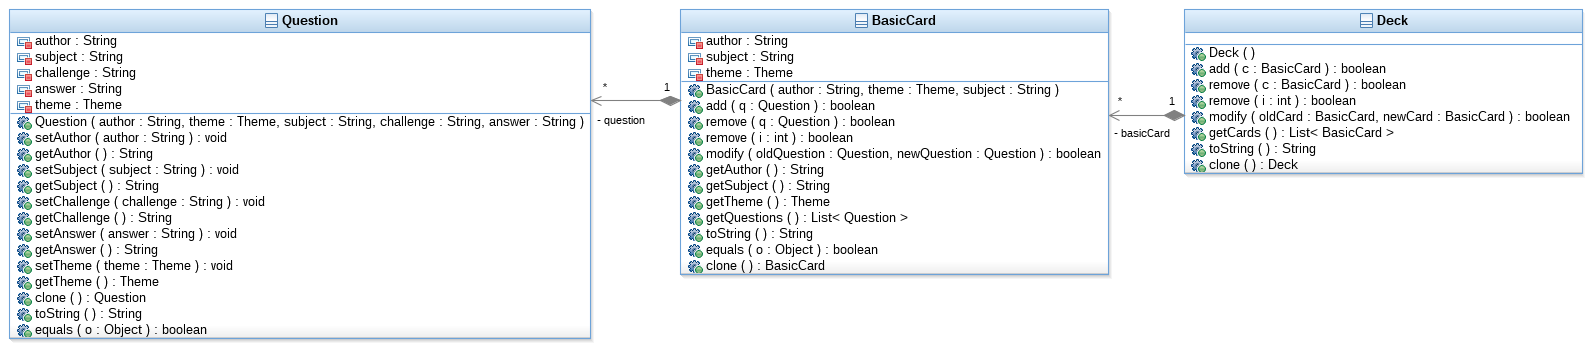
\includegraphics[width=\textwidth]{ttmc_modele.png}
	\caption{Diagramme du modèle}
	\label{fig:diag_modele}
\end{figure}

Le modèle est composé principalement de 3 classes et une énumeration.
La premier classe que l'on va analyser est la classe \verb|Question|.
Une question est caractérisée par:
\begin{itemize}
\item un auteur
\item un sujet
\item une question
\item une seule réponse possible
\item un thème
\end{itemize}

Étant donné que cette classe ne fait pas de manipulations particulières elle est principalement composée de \verb|Setters| et \verb|Getters| propre à chaque attribut.
Afin de vérifier un cas de similitude entre deux questions, une fonction \verb|equals()| a été écrite.
Pour permettre une nouvelle instantiation de cette classe, une fonction \verb|clone()| a été mise en place.
Enfin, afin d'assurer une sortie facilement lisible à l'être humain, la fonction \verb|toString()| a été surchargée.\\

La deuxième classe qui caractérise le modèle est la classe \verb|BasicCard|.
Une carte dans notre jeu est caractérisée par les attributs suivants:
\begin{itemize}
\item un auteur
\item un sujet
\item un thème
\end{itemize}
Une \verb|BasicCard| fait des manipulations plus complexes que la classe \verb|Question|.
Une carte est \textbf{composée} de une ou plusieurs questions, ceci doit être capable d'ajouter des nouvelles questions a sa liste, de supprimer des questions, ou remplacer une question par une autre.
Tout comme la classe \verb|Question|, la classe \verb|BasicCard| est aussi composée de \verb|Setters| et \verb|Getters|.
La classe \verb|BasicCard| aura aussi sa propre fonction \verb|equals()|, qui permettra la vérification de doublons, lors de l'ajout de ceci dans un deck.
Sa propre fonction \verb|toString()| affichera bien les attributs qui la caractérisent ainsi que les questions qui la composent.
La méthode \verb|clone()|, qui sert tout de même a renvoyer une nouvelle instance de la carte, servira principalement à assurer la \textbf{composition} entre la classe \verb|Deck| la classe \verb|BasicCard|.\\

La troisième et dernière classe qui fait des manipulations toutes autant complexes est la classe \verb|Deck|.
Cette classe n'a pas d'attributs qui la caractérisent car elle sert principalement à stocker les cartes.
Tout comme la classe \verb|BasicCard| cette classe aussi doit être capable d'ajouter des nouveaux éléments à sa liste, doit pouvoir supprimer un ou plusieurs éléments et doit être capable de remplacer une élément par un autre.
Étant donné que cette classe ne sera pas stockée dans une autre classe, elle ne nécéssite pas de \verb|equals()|.
Tout comme les autres classes, elle possède aussi son propre \verb|toString()| qui lui permettra d'afficher toutes les cartes qui seront stockées à l'intérieur de sa liste.
Afin d'assurer la sécurité de ses données nativement introduites, il est possible de cloner le deck grâce à la fonction \verb|clone()| qui créera une nouvelle instance de la classe \verb|Deck| originale, copiera toutes les cartes présentes dans le deck original et les ajoutera dans la liste de la nouvelle instance.

\newpage
\subsubsection{La vue}
\begin{figure}[h]
	\centering
	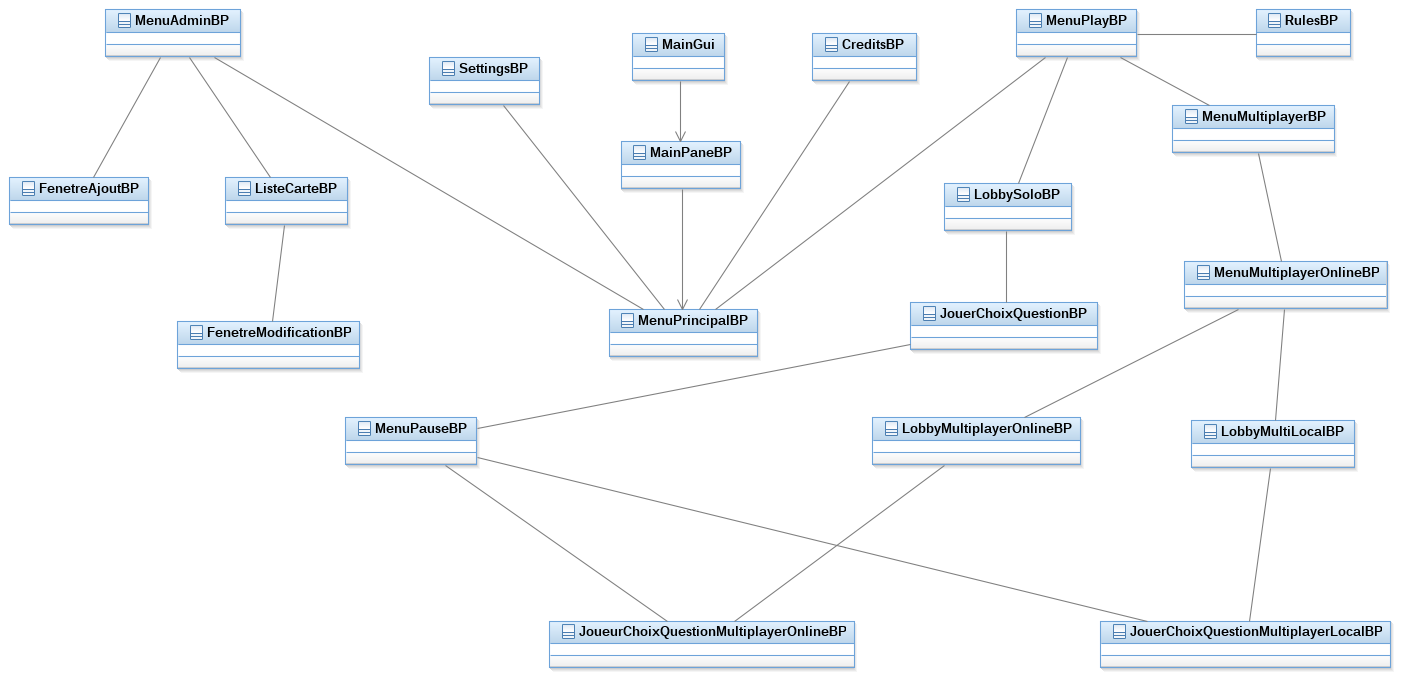
\includegraphics[width=\textwidth]{ttmc_vue.png}
	\caption{Diagramme de la vue}
	\label{fig:diag_vue}
\end{figure}

Lors du lancement du programme, l'instantiation de la vue est faite de manière linéaire jusqu'à ce que la classe \verb|MenuPrincipalBP| ne soit pas instanciée.
La classe \verb|MainGui| va charger les différents paramètres qui caractérisent la fenêtre:
\begin{itemize}
\item la largeur et la hauteur de la fenêtre
\item la musique qui sera jouée en arrière-plan
\item la langue qui sera visualisée
\end{itemize}
Une fois que les paramètres seront chargés, la classe \verb|MainPaneBP| va commencer à instantier les différentes parties qui composent le menu principale:
\begin{itemize}
\item le menu principale même
\item le menu pour commencer une partie
\item le menu pour accéder au panneau d'administration
\item le panneau des paramètres de la fenêtre
\item le panneau des crédits
\end{itemize}
Une fois que ces parties seront instanciées, si l'utilisateur décide d'accéder au menu pour jouer, il se trouvera devant un menu qui lui permettra de:
\begin{itemize}
\item lancer une partie solo
\item lancer une partie en multijoueur
\end{itemize}
Si son choix est celui de lancer une partie solo, une fois avoir inséré son pseudonyme, il sera introduit à une \enquote{lobby} ou \enquote{salle d'attente}, partie du menu qui lui permettra de faire les choix suivants:
\begin{itemize}
\item lancer une toute nouvelle partie avec le deck qui a été chargée dès le lancement du programme
\item lancer une partie en chargeant un deck de son choix
\end{itemize}
Indépendamment de son choix, il sera lancé vers \verb|JouerChoixQuestionBP|, fenêtre dans laquelle il ménera l'entièreté de sa partie.
Si son choix était de lancer une partie multijoueur, alors il aurait été introduit à un menu avec les choix suivants:
\begin{itemize}
\item lancer une partie multijoueur en local
\item lancer une partie multijoueur en ligne
\end{itemize}
S'il décide de lancer la partie en multijoueur local, il lui sera demandé d'insérer le nombre de joueurs qui participeront à la partie.
Une fois que chaque joueur a introduit son pseudonyme, tout comme pour la partie solo, il seront tous envoyés dans une \enquote{lobby} ou \enquote{salle d'attente}.
Cette solution permet aux joueur de relancer une partie sans devoir réinsérer leurs respectifs pseudonymes à nouveau.
Lorsque la \enquote{lobby} aura chargé, ils seront capables de lancer une nouvelle partie, lors du lancement, tous les joueurs seront renvoyés vers \verb|JouerChoixQuestionMultiplayerLocalBP|, classe qui laissera dérouler l'entièreté de leur partie.
Dans le cas du multijoueur en ligne, l'utilisateur sera invité à choisir entre:
\begin{itemize}
\item héberger un serveur
\item rejoindre un serveur
\end{itemize}
Si l'utilisateur décide d'héberger une partie, il lui sera demandé d'introduire le nombre de joueur qui participeront à la partie, ce dernier équivaudra au nombre maximal de joueurs qui sauront rejoindre le serveur.
Dans le cas où l'utilisateur décide de rejoindre un serveur, il sera invité à introduire son pseudonyme et l'adresse du serveur à rejoindre.
Indépendamment s'il hébérge ou rejoint un serveur, il sera introduit à une \enquote{lobby} ou \enquote{salle d'attente} dans laquelle il y aura aussi les autres joeurs lorsqu'ils rejoindront le serveur.
Dans ce \enquote{lobby}, les joueurs qui rejoindront seront introduits à une fenêtre qui leur permettra de quitter le serveur et intéragique avec les autres joueurs à travers une \enquote{chat box}, seulement celui qui hébérge la partie peux activer \verb|JouerChoixQuestionMultiplayerOnlineBP|.
Indépendamment du type de partie choisi, tout utilisateur sera capable de mettre en pause la partie à travers la touche \verb|ESCAPE|, ceci leur permettra d'accéder au \verb|MenuPauseBP|.
Ce dernier, leur permettra de quitter la partie et revenir au \enquote{lobby} ou reprendre la partie mise en pause.\\
Ceci est tout pour la partie \enquote{jeu} de la vue.\\
Une autre partie de la vue que l'utilisateur sait accéder depuis \verb|MenuPrincipalBP| est \verb|MenuAdminBP|.
Dans ce panneau, l'utilisateur sera capable d'accéder à une fenêtre qui lui permettra d'ajouter une toute nouvelle carte à son deck, ainsi qu'à une fenêtre qui lui montrera la liste de cartes qui composent son deck: \verb|ListeCarteBP|.
En cliquant sur une des cartes sur la liste, il sera renvoyé vers une autre fenêtre: \verb|FenetreModificationBP| qui lui permettra de modifier la carte choisie s'il le désire.\\
Les autre fonctionnalités qui caractérisent la vue sont: \verb|SettingsBP| et \verb|CreditsBP|.
\verb|SettingsBP| permet à l'utilisateur de changer les paramètres qui caractérisent le jeu et la fenêtre.\\
\verb|CreditsBP| lui montrera les informations sur les développeurs du jeu ainsi que les musiques utilisées et toutes les personnes qui ont contribués aux traductions.

\subsubsection{Les exceptions}

\begin{figure}[h]
	\centering
	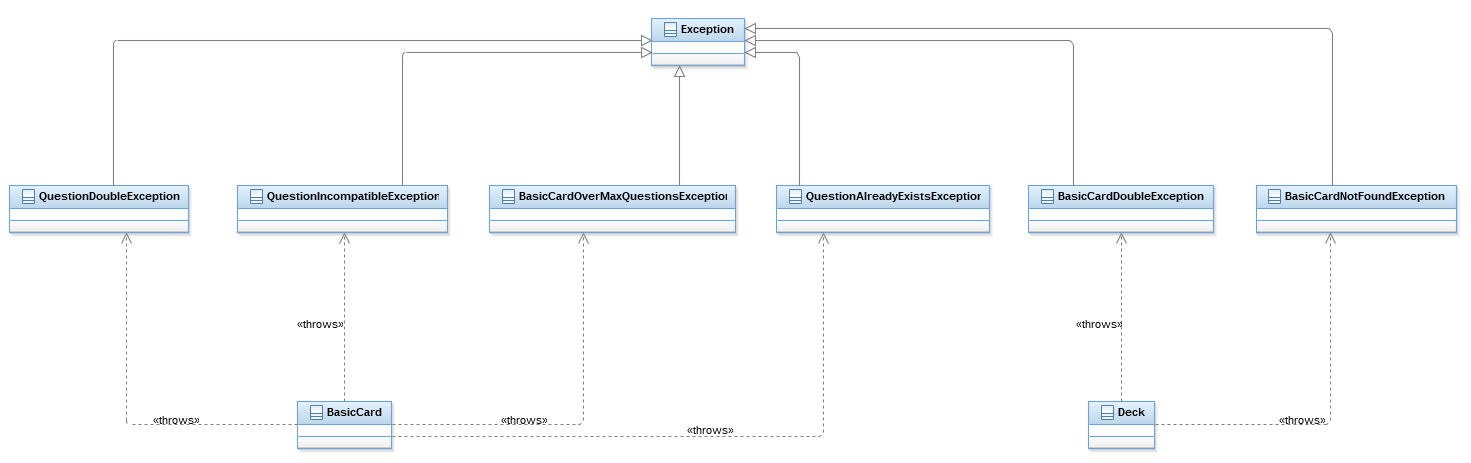
\includegraphics[width=\textwidth]{ttmc_exception.png}
	\caption{Diagramme des exceptions}
	\label{fig:diag_exception}
\end{figure}

